\chapter{Application Design and Requirements}
\label{ch:ApplicationDesignAndReq}

This chapter will describe the current system of the Blinky mobile application, including the backend server, the clients  and the requirements for the smart contract integration.

\section{System overview and technical terms}

The Blinky mobile application is a cross-platform client written in React Native \citep{ReactNative}, a framework to develop mobile applications using the JavaScript programming language. The usage of the application enables users to register, create a Cost-Split event that happened after he/she paid for one event for everyone and need to split the cost equally and get the part of the money which others owe.

\begin{figure}
    \centering
    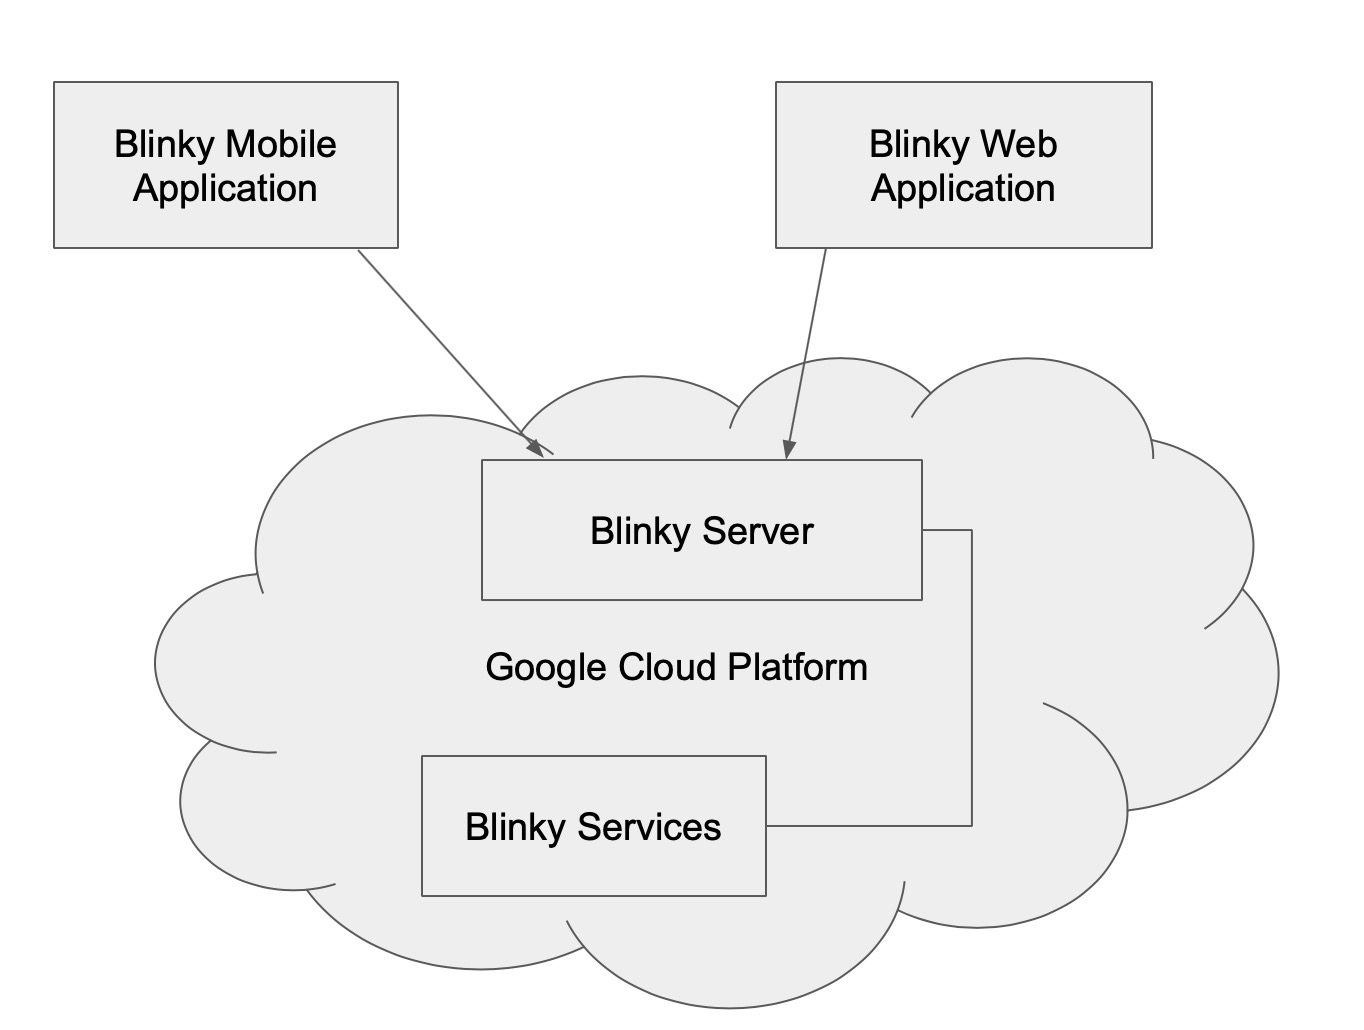
\includegraphics[width=\linewidth]{blinky_system_architecture.jpg}
    \caption{Blinky system architecture}
    \label{fig:blinky_system}
\end{figure}

Users of the Blinky Application can also generate a web URL to share that split cost to friends or relatives. The URL acts as an interface that non-Blinky users can also interact with the services even though they do not have an account. The URL leads to a web application written in React library, which helps building user interface.

Figure \ref{fig:blinky_system} represents the system powering Blinky and where those system are deployed to. 

\section{Application use cases}

The Blinky application was created with the main aim was to help its users to calculate the shares between friends after someone has paid before hand, to ensure a fair and equal split. The application also tries to free users from sticking to one particular payment solution, which allows user to register their preferred payment solution details and later user can share that details together with the calculation details to their friends. Their friends then see the calculation details and take the shared payment method in order to make the payment back to user. From here until the end of this thesis, each of this series of actions from user will be referred as a "Cost-Split" event.

\section{REST API}

The clients, mobile applications and the web application  can communicate with the backend service with a Representational State Transfer (REST)  \citep{REST} Application Programming Interface (API). Data is represented and sent through Javascript Object Notation (JSON).

Users in the mobile application will be granted access right determined by a JSON Web Token (JWT) which can be used in the header of every request to the back-end service. The token contains the user's information which  can easily be used to identify and authenticate them.

The Blinky RestAPI Service will provide an interface for the mobile application so that users can create, edit and delete Cost-Splits, and then invite participants, add expenses to split. Each time a Cost-Split, participant or expense is created on the server, an unique identifier will be generated as an integer and attached to that object. The identifier is then also be used to refer to that object in later actions of its lifetime as well as to delete.
\label{blinkyAPI}

\section{Requirements}
\label{section:requirements}

The requirements for integration with the Ethereum smart contract include:

\begin{itemize}
    \item Generate a new data slot on the smart contract state when a new Cost-Split is created on the application
    \item Increment the data slot with new data each time a Cost-Split is edited with a new user's action such as changing expenses' detail, participants in the Cost-Split, generate an URL, or someone interacted with that URL
\end{itemize}

The requirements are chosen because they depict the common scenarios of transparency between small Cost-Split of a party, such as how much each has to pay, who did declare to have paid.

\subsection{Generating data slot on smart contract}

The desired smart contract will hold a map which contains each Cost-Split's happened event. Each Cost-Split will have its own memory space to store events in a chronological order. Whenever a new event is fired on the client mobile application, a function inside the smart contract should be called provided with the content of the event such as the description, time stamp, user's identifier. The function will then process the input-ed data and append it into that Cost-Split's memory space.

\subsection{Provide a data-retrieval interface for user}

Users of the Blinky application also have the right to request their data in a readable manner, an user-friendly interface. This means that the application will need to provide a function that will represent user and request the data about the user-desired Cost-Split saved on the smart contract. The requested data should also be formatted into a reading-friendly that they can also use as a mean of proof for the action taken by him or anyone interacted with the shared Cost-Split.

\section{Asymptotic Notation}

In order to measure the performance of an algorithm or a computer operation, asymptotic notation is used \citep{AlgorithmAndDataStructure}. In general terms, it is a theoretical framework to measure an algorithm's operation taken to complete the task given a number of inputs. For example, if there is \texttt{n} inputs and the algorithm needs to do \texttt{n} operations on each input, the total number of operations needed to complete the task is \texttt{n * n}, which means it will be exponentially proportional to the number of inputs. In asymptotic notation, only the highest order of operations is taken. From the last example, if the number of operations needed is \texttt{n * n + 2n} then the asymptotic notation is still \texttt{n * n} since it carries order of 2.